\debut{Emile Martinez}{}{Représentation des nombres en binaires}{}

\section{Circuits booléens}

\subsection{Porte logique}

Les circuits d'un ordinateur manipulent des bits qui correspondent en interne à des tensions électriques. 


\begin{definition}
	Une porte logique est une fonction qui prend un ou plusieurs bits en entrée et qui renvoie un bit en sortie. 
\end{definition}

\begin{personalise}[Schéma]
	\begin{tabular}{ccc}
		\begin{circuitikz} \draw
			(0,0) node[and port] (a) {}
			;  
		\end{circuitikz} & \begin{circuitikz} \draw
			(0,0) node[or port] (a) {}
			;  
		\end{circuitikz} & \begin{circuitikz} \draw
			(0,0) node[not port] (a) {}
			;  
		\end{circuitikz} \\
		ET & OU & NON
	\end{tabular}
\end{personalise}

\begin{proposition}
	On peut composer les portes logiques, et scinder un fil : on crée alors des circuits booléens. Attention, on ne doit pas créer de boucles dans les circuits.
\end{proposition}

\begin{exercise}
	Exprimer la porte OU à l'aide des portes NON et ET.
\end{exercise}

\subsection{Expressivité}

\begin{definition}
	On définit inductivement l'ensemble EB des expressions booléennes par :
	\begin{itemize}[label=]
		\item Cas de base : $\top, \bot, x\in V$ (où $V$ est un ensemble de variable)
		\item Constructeurs : $\neg$ unaire, $\wedge$ et $\vee$ binaires
	\end{itemize}
\end{definition}

\begin{rem}
	Cela représente exactement les circuits booléens, où seuls les fils initiaux peuvent être dupliqués
\end{rem}

\begin{definition}
	Une valuation est une fonction $\sigma :V \to \{0,1\}$.
	\\
	\\
	On définit alors $[\,]_\sigma$ : $EB \to \{0, 1\}$ par induction sur EB par :\begin{itemize}[label=$\bullet$]
		\item $[\bot]_\sigma = 0$, $[\top]_\sigma = 1$ et $[x]_\sigma = \sigma(x)$ pour $x \in V$
		\item $[e_1 \vee e_2] = \max([e_1]_\sigma, [e_2]\sigma)$
		\item $[e_1 \wedge e_2] = \min([e_1]_\sigma, [e_2]\sigma)$
		\item $[\neg e_1]_\sigma = 1-[e_1]_\sigma$
	\end{itemize}
\end{definition}

\begin{rem}
	Cela revient à simuler l'exécution d'un circuit booléen.
\end{rem}

\begin{theorem}
	Pour toute fonction $f : \{0, 1\}^n \to \{0, 1\}$, il exsite une expression booléenne e ayant pour variables $\{x_1, \dots, x_n\}$ tel que pour tout $(b_1, \dots, b_n)\in\{0,1\}^n$, en prenant $\sigma$ tel que $\sigma(x_i) = b_i$ on ait alors $[e]_\sigma = f(b_1, \dots, b_n)$
\end{theorem}

\paragraph{Développement :} Preuve du théorème précédent et discussion autour de la complexité

\begin{personalise}[Conclusion]
	Les circuits booléens permettent d'exprimer toutes les fonctions que l'on pourrait vouloir calculer
\end{personalise}

\subsection{Introduction du temps}

Notre ordinateur est donc composé de circuits booléens. Néanmoins, on voudrait pouvoir brancher les circuits booléens entre eux (ce qui posent problème car les portes logiques ne changent pas de valeurs instantanément) et avoir de la rétroaction (ce qui est interdit).

\begin{idee}
	On introduit alors des briques de mémoire dans un ordinateur (registre) et une horologe (un tic tac). Les liens entre les différentes circuits ne se font alors que à travers des registres, qui se mettent à jour en même temps grâce à l'horologe. Ainsi, on a jamais de réelles boucles.
\end{idee}

\begin{rem}
	Les registres sont les plus petites unités de mémoire d'un ordinateur.
\end{rem}

\begin{example}
	Compteur sur 8 bits, faisant +1 à chaque tac du tic tac. \raisebox{-0.5\height}{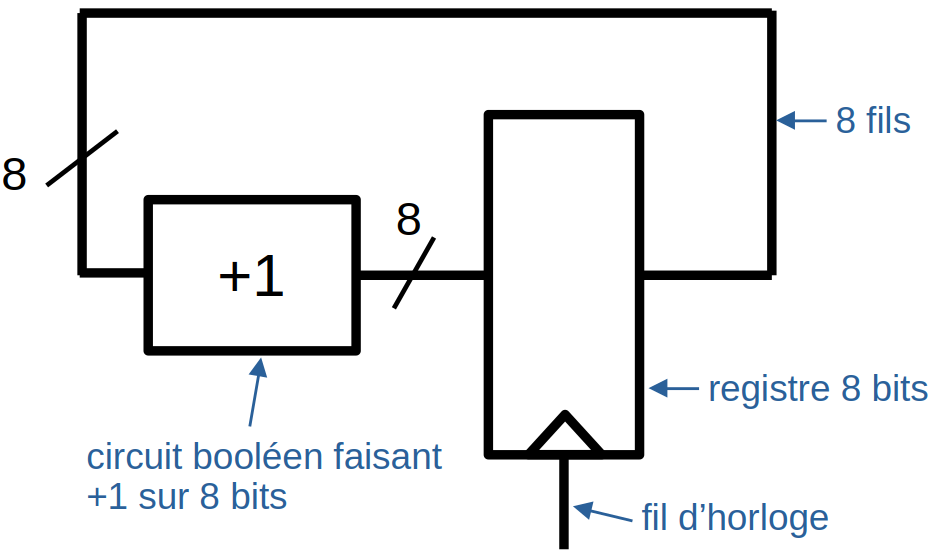
\includegraphics[width=0.4\linewidth]{lecon/23-archi-assembleur/compteur.png}}
\end{example}

\begin{rem}
	La fréquence de l'horloge détermine donc le temps minimal pour faire une opération dans un ordinateur. C'est ce que l'on dit quand on parle de processeur 4GHz (4 milliards de tac par secondes)
\end{rem}

\section{Modèle de Von Neuman}

\subsection{Le modèle}

\begin{definition}
	Une instruction est une opération à effectuer par le processeur sur des éléments de mémoire de l'ordinateur (registre, cache, RAM, disque dur, etc...).
\end{definition}

\begin{principe}
	Un ordinateur passe alors son temps à exécuter des instructions (qui modifie l'état de la mémoire)
\end{principe}

\begin{definition}
 	Le modèle de Von Neumann décrit le fonctionnement d'un ordinateur constitué : \begin{itemize}[label=$\bullet$] 
		\item d'un processeur qui lit les instructions en mémoire et les exécute. Il accède à la mémoire par blocs appelés mots mémoire. Pour cet accès, le processeur utilise un registre appelé compteur ordinal (Program Counter ou PC) qui contient une adresse en mémoire.
		\item La mémoire RAM adressé qui contient les programme à exécuter et les données. 
		\item Les périphériques d'entrée (clavier, souris, disque dur) et de sortie (écran, disque dur, haut parleur).
	 \end{itemize}
\end{definition}

\begin{rem}
	Une des spécificités de ce modèle est que les instructions sont des données comme les autres.
\end{rem}

\begin{personalise}[Schéma][Modèle de Von Neumann] CPU = processeur
	\begin{center}
		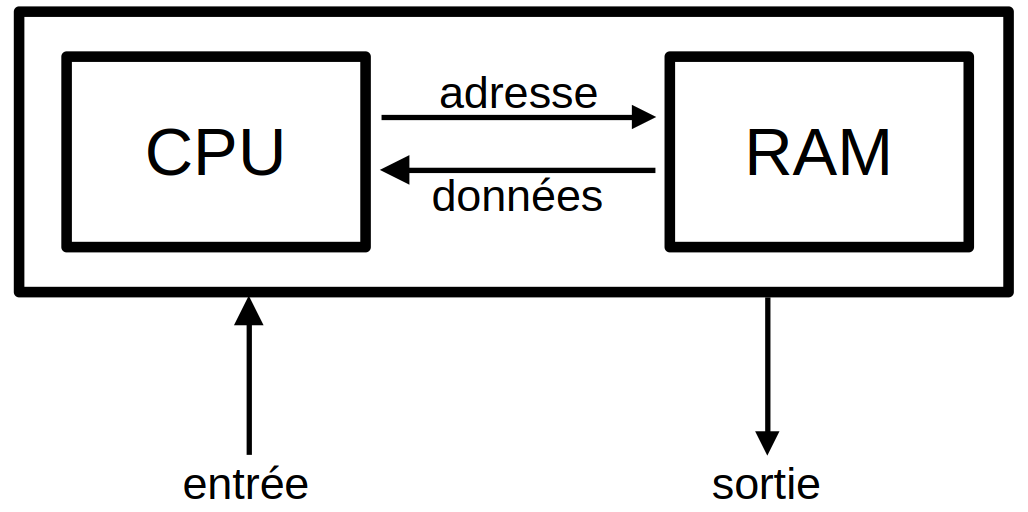
\includegraphics[width=0.5\linewidth]{lecon/23-archi-assembleur/modele_neumann.png}
	\end{center}
\end{personalise}

\begin{definition}[Cylce de Von Neumann]
	\begin{enumerate}
		\item \label{23-point1-cycle} Lire le mot mémoire qui commence à l'adresse PC
		\item Interpréter ce mot mémoire comme une instruction et l'exécuter
		\item Augmenter le PC pour passer à l'instruction suivante
		\item Retourner au \ref*{23-point1-cycle}
	\end{enumerate}
\end{definition}

\begin{rem}
	Quand vous avez plusieurs coeurs, il y a simplement plusieurs processeurs en parrallèle.
\end{rem}

\subsection{Registres et mémoire adressable}

Dans le modèle, la mémoire n'est pas dans le processeur. C'est la mémoire adressable (accessible par adresse).\\

Néanmoins, il y a aussi de la mémoire dans le processeur. Ce sont les registres. Quand un processeur veut exécuter une opération, il doit alors stocker les données dans des registres (les avoir en mémoire, sous la main), faire l'opération (et comme il doit stocker le résultat, le mettre dans un registre), puis renvoyer le résultat à la mémoire.

\begin{rem}
	Un processeur possède un registre stockant la valeur de PC.
\end{rem}

\section{Jeu d'instruction}

\subsection{Définition}

\begin{definition}
	Une instruction machine est une séquence de bits que le processeur peut interpréter et exécuter. Un jeu d'instructions (ISA) définit quelles sont les instructions supportées par le processeur, et la façon dont elles sont représentées en mémoire. L'ensemble de ces instructions machines forment le langage reconnu par le processeur, appelé langage machine. 
\end{definition}

\begin{rem}
	Tous les codes dans n'importe quel langage de programmation (exemple Python) doivent être traduits en langage machine pour être exécutés par le processeur. 
\end{rem}

\begin{proposition}
	En général, les jeux d'instructions gèrent les opérations suivantes : \begin{itemize}[label=$\bullet$]
		\item lire le contenu d'une case mémoire dans un registre, écrire le contenu d'un registre dans une case mémoire 
		\item opérations arithmétiques ou logiques (addition, et bit à bit, etc...)
		\item se déplacer dans le programme que l'on exécute (sauts)
	\end{itemize}
\end{proposition}

\begin{rem}
	Il exsite de nombreux ISA différents. On peut les diviser en deux catégories principales :
	
	CISC (complex instruction set computer) : plus d'instruction pouvant faire plus de choses mais donc plus longues (ex. x86 sur la plupart des ordinateurs)
	
	RISC (reduced instruction set computer) : moins d'instruction mais plus rapide et facile à implémenter (ex : RISC-V, ARM sur des téléphones).
\end{rem}

\subsection{Langage assembleur}

Une instruction est représentée en mémoire par un code en binaire. Par exemple, si les trois premiers bits sont des 0, on doit faire une opération arithmétique, puis si les deux suivants sont des 1, on fait une addition, etc. Néanmoins, cela est très peu lisible par l'être humain.

\begin{definition}
	Le langage assembleur représente le langage machine sous une forme lisible par un humain. C'est le langage de programmation de plus bas niveau.
\end{definition}

\begin{example}
	Exemple d'instruction classique : \begin{itemize}[label=$\bullet$]
		\item \texttt{load $r_i$ [$r_j$]}  : mets le contenu à l'addresse contenu dans $r_j$ dans le registre $r_i$
		\item \texttt{store $r_i$ [$r_j$]} : mets le contenu du registre $r_i$ dans la case d'adresse contenu dans $r_j$
		\item \texttt{add $r_i$ $r_j$ $r_k$} : ajoute le contenu des registres $r_i$ et $r_j$ pour le mettre dans le registre $r_k$
		\item \texttt{iload $r_i$ $x$} : mets la valeur $x$ dans le registre $r_i$
		\item \texttt{mv $r_i$ $r_j$} : mets la valeur du registre $r_i$ dans le registre $r_j$.
	\end{itemize}
\end{example}

\begin{example}
	Traduction en langage assembleur du code python «\texttt{z = x + y}»
	\begin{lstlisting}
iload <@$r_1$@> <@(adresse de x)@>
load <@$r_2$@> [<@$r_1$@>]
iload <@$r_1$@> <@(adresse de y)@>
load <@$r_3$@> [<@$r_1$@>]
add <@$r_1$@> <@$r_2$@> <@$r_3$@>
iload <@$r_1$@> <@(adresse de z)@>
store <@$r_2$@> [<@$r_1$@>]
	\end{lstlisting}
\end{example}

\begin{rem}
	Pour pouvoir exécuter des boucles et les si, on introduit de nouvelles instructions : \begin{itemize}[label=$\bullet$]
		\item \texttt{bge $r_1$ $r_2$ N} : va à la ligne $N$ si $r_1 \geq r_2$;
		\item \texttt{bgt}, \texttt{ble}, \texttt{beq}, \texttt{blt} (pour $>$, $\leq$, $=$, $<$)
		\item \texttt{jump $N$} : saute à la $N$-ième instruction du programme
	\end{itemize}
\end{rem}

\begin{example}
	Pour \texttt{while (i < n): i = i + 1}
	\begin{lstlisting}
0. iload <@$r_1$@> <@(adresse de x)@>
1. iload <@$r_2$@> <@(adresse de n)@>
2. load <@$r_2$@> [<@$r_2$@>]             // contient n
3. load <@$r_3$@> [<@$r_1$@>]             // contient i
4. bge <@$r_3$@> <@$r_2$@> 9
5. iload <@$r_4$@> 1
6. add <@$r_3$@> <@$r_3$@> <@$r_4$@>
7. store <@$r_3$@> [<@$r_1$@>]            // mettre à jour i
8. jump 3
9.
	\end{lstlisting}
\end{example}

\begin{rem}
	On peut faire beaucoup d'optimisation (par exemple en ne stockant $i$ que à la fin). Ce sont là d'importants sujet d'études (en compilation)
\end{rem}

\section{Gestion de la mémoire à plus haut niveau}

\begin{com}
	La raison de cette partie n'est pas uniquement de nous donner un développement mieux, mais également que c'est l'étape d'après dans la construction d'un ordinateur. Ici on commence à poser les premières briques du dessus. Surtout que c'est une étape cruciale de la compilation (passage de langage de plus haut niveau au code machine). Donc en tant qu'ouverture, tout en utilisant le langage assembleur ca parait cohérent.
\end{com}

Quand on exécute un programme qui n'est pas dans un langage assembleur, on a souvent besoin d’instruction de plus haut niveau, nous permettant d'allouer des variables, de faire des appels de fonctions imbriqués, etc. ce qui n'est à priori pas disponibles dans le langage assembleur tel quel.\\

Il faut alors traduire ces instructions de plus haut niveau en langage assembleur (i.e. compiler)

\begin{principe}
	Lors de l'exécution d'un processus, un espace mémoire en RAM lui est réservé. 
\end{principe}

\begin{minipage}{0.2\linewidth}
	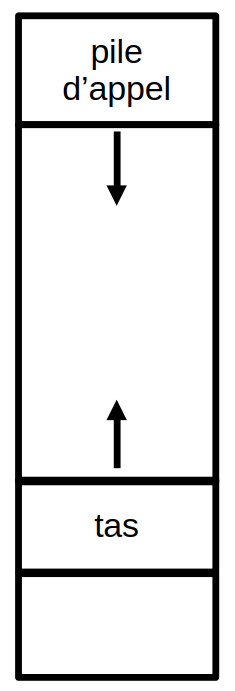
\includegraphics[height=6cm]{lecon/23-archi-assembleur/pile.png}
\end{minipage} \qquad
\begin{minipage}{0.6\linewidth}
	\begin{principe}    
		Le tas gère les données accessibles depuis tout le programme (malloc).
		
		Dans la pile, on met les variables locales à une fonction. A chaque nouvel appel, on empile de l'espace pour l'appel de fonction, que l'on enlève quand on return.
	\end{principe}
\end{minipage}

\paragraph{Développement :} Explication de la pile d'appel et implémentation en assembleur